\section{Introduction}
Path planning is an important and long studied problem in AI, and 
it is a problem which finds common application in different real-world
settings such as robotics and computer games.
When the problem appears in practice, it is often assumed that the
input environment can be modelled as a two-dimensional \emph{gridmap}
that is made up of traversable and non-traversable cells.
Despite significant improvements in the recent literature, path planning on 
gridmaps remains an active area of research. 
This is demonstrated, for instance, by the interest shown in the Grid-based 
Path Planning Competition GPPC~\cite{DBLP:conf/socs/SturtevantTTUKS15}.

Among the fastest currently known methods, for computing optimal grid paths,
is a family of techniques known as Compressed Path Databases 
(CPDs)~\cite{botea-aiide11,bh-ppcap-13}.
Each CPD is simply a data structure that tells, for any start location 
$s$ and any target location $t$, which is the optimal first move from $s$ to $t$.
Finding a shortest path using such a database is straightforward: 
simply look up the optimal first-move toward target and execute that move, 
repeating as necessary until the target is reached.

%Created offline but exploited online, CPDs can be used to quickly extract any 
%optimal path or any optimal prefix\footnote{By optimal prefix we refer to a 
%type of query that seeks only the first $k$ steps of an optimal path. 
%Such queries arise when planning time is limited or when planning and execution
%are interleaved.} 
%without the need for state-space search.
%
%CPDs are created offline by executing a series of independent Dijkstra searches: 
%one from each \change{source} node $s$ on the graph \change{underlying the gridmap}. 
%At the completion of each Dijkstra search the first-move data is losslessly compressed 
%into a smaller format and written to disk. Later, during a subsequent online phase, the 
%entire database is loaded into main memory and used to compute shortest paths.
%
%The Dijkstra algorithm is slightly modified to output
%a set of optimal \change{first} moves, as opposed to distances.
%More specifically, this provides all
%%\pjs{all? Resp Adi: Yes, thanks for pointing out. Text modified.}
%optimal \change{first} moves from the source at hand $s$ towards any
%other node $t$ on the \change{underlying} graph. 
%A compression technique selects one \change{first} optimal move from $s$ to each target,
%and compresses the corresponding string of move symbols.
%%The set of optimal moves is compressed. 

%To find a shortest path CPDs employ a simple procedure: 
%look up the optimal first-move toward target and then execute that move; 
%a process which is repeated again and again until the target is reached.

The principal advantage of CPDs is the speed performance: optimal paths can be found
quickly and without any state-space search.
Meanwhile optimal prefixes (i.e., the first several steps
of an optimal path) can be found faster still.
This feature is important to reduce the {\em first-move lag}, where
an agent needs to wait until it knows in which direction to start
moving.
%CPDs identify optimal prefixes using just a small number of lookups.
In contrast, consider that search-based methods can only know an optimal 
prefix once they know the entire path.

%CPDs can also be used to quickly provide any prefix of an optimal
%path. This is important to reduce the so-called first-move lag, where
%an agent needs to wait until it knows in which direction to move.
%Many other pathfinding techniques for example, including search-based methods 
%derived from A*~\cite{hart68formal} %and approaches using A*,
%know the first optimal move only when they know the entire
%solution. By contrast, CPDs identify such moves faster 
%and independently from the rest of the path.

The main drawback of CPDs is build cost:
each database requires an all-pairs pre-compute with space and time
being worst-case quadratic in the size of the input 
graph; i.e., we need to run one Dijkstra search per node in the 
graph and then compress and store the result.
Researchers in this area typically prioritise fast online performance
and for this reason works tend to focus on reducing the size of 
the database, so it can fit in working memory~
\cite{strasser-et-al-2014,DBLP:conf/aips/SalvettiBSG17,icaps19b},
or they focus on improving lookup performance, so that moves can be 
extracted sooner~\cite{DBLP:conf/aips/SalvettiBGHS18}.

In this paper we consider a new bounded-suboptimal take on CPDs which 
cuts the time required for precomputation. The same approach can 
also reduce storage costs and yield faster online performance -- 
all in exchange for a small amount of additional cost per extracted path.
Our idea involves selecting from the input map a subset of nodes $C$,
which we call {\em centroids}, such that every node is at most a 
path distance $\delta$ from some centroid $c \in C$. 
During precomputation we store first move data from every node 
in the graph to every centroid. The entire procedure requires at most
$|C|$ offline instantiations of Dijkstra search. More, the resulting
database is sufficient to determine a bounded suboptimal path,
from any node $s$ to any other node $t$.
%The resulting database can be used to extract a path from any start 
%node $s$ to any target node $t$ as follows: we simply determine the 
%centroid $\centroid(t)$ of the target and construct an optimal path 
%from $s$ to $\centroid(t)$ and then from $\centroid(t)$ to $t$.
We give a theoretical description of the method and show that,
for a given value of $\delta$, the cost of each extracted path is at 
most $2\delta$ larger than optimal, with $\delta$ being an input
parameter.  

In experiments, we test this idea with different values of $\delta$ and 
with different compression schemes.
Results on standard grid benchmarks indicate order
of magnitude reductions in preprocessing times, and up to several factors
improvement in database size and lookup speed. We also show that, in many 
cases, the suboptimality cost per path is substantially smaller than the 
guaranteed upperbound.
%
%
%%A straightforward idea to reduce the size of CPDs
%%stored arises if we are willing to relax the requirement to find an optimal path from start to target.
%We select a set $C$ of \emph{centroids}, points in the map, so that each point is within a distance $\delta$
%from some centroid.  We can straighforwardly build a mapping from point $t$ to its centroid $\centroid(t) \in C$.
%In the CPDs for each start point 
%$s$ we only store the optimal move to each centroid $C$ rather than
%to all other points.  We can now construct a path from arbitrary start $s$ to target $t$ by
%determining the centroid $\centroid(t)$ of the target, using the CPDs to construct an optimal path
%from $s$ to $\centroid(t)$, and using the CPDs to construct an optimal path from $t$ to $\centroid(t)$.
%Conjoining these two paths we get a path from $s$ to $t$ which is at most $2\delta$ longer than the optimal path.
%Since the CPDs only record optimal first moves to each centroid $c \in C$ rather than each possible
%target $t$ they can be smaller.
%
%Unfortunately, this idea fails. Figure~\ref{fig:fwd0-fwdc} shows the size of a full CPD divided by the size of the CPD build using centroids with radii $\delta = $ 2,4,8,16,32 and 64.
%We can clearly see that we dont get the compression we expect. Even with a radius
%of 64, where we typically have the number of centroids $|C|$ is around one thousandth
%of the number of cells in the map the median compression
%of the full CPD is less than 2.  
%Note that some CPDs for centroid in fact require more memory than a full CPD since we need to store the centroid map in addition.
%\pjs{The line 1.0 must appear in the graph and be marked!}
%
%\begin{figure}
%    \centering
%    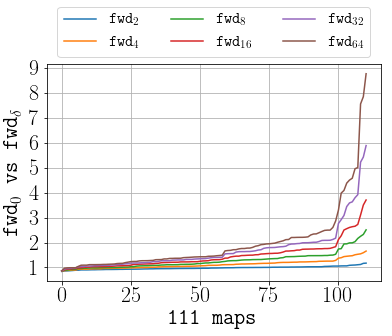
\includegraphics[width=\columnwidth]{pic/fwd0-fwd.png}
%    \caption{Memory requirement of a full CPD divided by memory requirement for a CPD for centroids with radius $\delta = 2,4,8,16,32,64$. The ratios for 111 maps are sorted from smallest to largest.}
%    \label{fig:fwd0-fwdc}
%\end{figure}
%
%
%The reason is that the run length encoding of a map for location $s$ to each target
%is not that much bigger than the run length encoding for location $s$ to just the centroids $C$.
%To overcome the problem we will introduce \emph{reverse CPDs}, where rather than store
%for each start location $s$ a map of the first move to get to any target $t$, we
%store for each target location $t$ a map of the first move to get there from start location $s$.
%
%We undertake a detailed evaluation on 
%gridmaps from Sturtevant's well known benchmark sets~\cite{sturtevant2012benchmarks}.
%
%
%The rest of this paper is organised as follows.
%In the next section, we present background material on CPDs
%and summarise existing work in the area.
%In Section~\ref{sec:bounded}, we formally define bounded sub-optimal path finding using centroids.
%In Section~\ref{sec:centroid}, given a map 
%how to choose centroids for a given $\delta$.
%In Section~\ref{sec:reverse}, we introduce 
%reverse CPDs which store information about the first move from any start position $s$ to a 
%given target $t$ as opposed to from a given start position $s$ to any target $t$. 
%We show how to improve compression of reverse CPDs.
%In Section~\ref{sec:results}, 
%we explain the experimental setup
%and give experimental results.
%Finally, in Section~\ref{sec:conclusion} we give the conclusions and mention future work.
%
%\sz{
%Strange! Section counter somehow messed up
%}
%
